
\documentclass[11pt]{article}


% Use wide margins, but not quite so wide as fullpage.sty
\marginparwidth 0.2in 
\oddsidemargin 0.1in 
\evensidemargin 0.1in 
\marginparsep 0.1in
\topmargin 0.1in 
\textwidth 6.5in \textheight 8 in
% That's about enough definitions

% multirow allows you to combine rows in columns
\usepackage{multirow}
% tabularx allows manual tweaking of column width
\usepackage{tabularx}
% longtable does better format for tables that span pages
\usepackage{longtable}
\usepackage{graphicx}
\usepackage{amssymb} % needed for math
\usepackage{amsmath} % needed for math 
\usepackage{color}
\definecolor{dkgreen}{rgb}{0,0.6,0}
\definecolor{gray}{rgb}{0.5,0.5,0.5}
\definecolor{mauve}{rgb}{0.58,0,0.82}
\usepackage{hyperref}  
\usepackage{listings}

\begin{document}

\author{İbrahim Burak Tanrıkulu, 21827852}
\title{BBM301 Programming Languages\\Fall 2020\\Assignment 1\\Evaluating a New Programming Language\\Assembly Language}
\maketitle

\section{What is Assembly? Why we use this language?}

\begin{itemize}
	\item { Every computer has a processor. Processors understand only machine language instructions. However, machine language is too obscure and complex. So, assembly language is designed. \href{https://www.tutorialspoint.com/assembly_programming/assembly_introduction.htm}{1}}
	\item { Assembly language is a low-level programming language that invented theoretically in 1947 by Kathleen Booth while working on the ARC2 at Birkbeck, University of London following consultation by Andrew Booth, John von Neumann and Herman Goldstine at Institute for Advanced Study. \href{https://en.wikipedia.org/wiki/Assembly_language}{2}}
	\item { Assembly languages helps programmers to write the human-readable code that is almost similar to machine language. Assembly language helps in providing full control of computer tasks. \href{https://www.educba.com/what-is-assembly-language/}{3}}
	\item { In the past, many programs and applications were written in assembly language to maximize the machine's performance. Today; C, Java, Python is widely used. Like assembly language, C/C++ can manipulate the bits at the machine level, but it is also portable to different computer platforms. There are C/C++ compilers for almost all computers. \href{https://www.pcmag.com/encyclopedia/term/assembly-language}{4}}
	\item { Assembly code is converted into executable machine code by an assembler. The conversion process is referred to as assembly.}
	\item { Different processors have different architecture or instructions and Assembly Language mainly consists of mnemonic processor instructions or data, and other statements or instructions. Thus, Assembly languages are hardware dependent; there is a different one for each CPU series. Sometimes, Assembly languages can be different on different operation systems because of system calls. }
	\item { Today, the learning of assembly language is still important for programmers. It helps in taking complete control over the system and its resources. By learning assembly language, the programmer is able to write the code to access registers and able to retrieve the memory address of pointers and values. Also Assembly language learning helps in understanding the processor and memory functions. }
	\item { I choosed Assembly language in this assignment. Because i am interested in computer architecture and microprocessors. I love to taking control of computer and doing whatever i want. I think Assembly and C language is very functional.} 
\end{itemize}

\section{Language evaluation criteria}

\begin{itemize}
	\item  {{\bf Readability \& Writability }}
	\newline In 1940's programmers were reading and writing machine codes directly. So assembly language provided convenience to programmers at that time. Because Assembly language was more readable and writable than machine code. But today, we are naming Assembly language as "low-level language". Assembly language is less readable and writable than high-level languages like C, Python, Java etc. . 
	\newline {\bf Simplicity:} There are nearly 2000 instructions in this language and instruction names are abbreviations of English words. We must use lots of instructions to do basic operations. Thus, I can easily say that Assembly language is not simple. 
	\newline {\bf Orthogonality:} Assembly language is orthogonal. Because one instruction can do one thing and can use nearly all adressing modes. For example; "add" instruction can take place between "register to register" or "memory to register" or "register to memory".
	\newline {\bf Data Types:} In Assembly language we define data with sizes (byte or word(2 bytes)). It doesn't matter what we store inside that memory. Also we can define array of bytes or words.  All of variables can defined by byte, word, doubleword, quadword or ten bytes. 
	\newline {\bf Syntax:} An assembly program can be divided into three sections: data, bss, text. Statements are entered one statement per line. Each statement follows the following format:
	\newline {\bf [label]   mnemonic   [operands]   [;comment]}
	\newline The fields in the square brackets are optional. A basic instruction has two parts, the first one is the name of the instruction (or the mnemonic), which is to be executed, and the second are the operands or the parameters of the command.
	\newline {\bf Abstraction:} Assembly language has no support for abstraction but we can use adressing for data abstraction, procedures or macros for process abstraction maybe.
	\newline {\bf Expressivity:} Assembly Language has flags that we can use in some instructions. JNZ instruction can be used for a loop. Also there are some instructions to do operations easily.
	\newline For example, "add ecx, 1" (ecx(a register) = ecx + 1) can be done with "inc ecx" .

	\item {{\bf Reliability}}
	\newline Reliability changes to assembler and assembler changes to architecture. In low-level assemblers (original assemblers) reliability is almost unavailable. But high-level assemblers are good at this. There is default size-checking and syntax-checking in all assemblers .
	\item {{\bf Cost}}
	\newline {\bf Training:} Assembly language is orthogonal but not simple. There are lots of instruction to learn but every instruction does one thing. Teaching all instructions may be hard but if you think the machine code, assembly is easier then that. Teaching assembly is better than teaching machine code, but worse than teaching high-level programming languages.
	\newline {\bf Writing:} Assembly language writing is easier than machine code writing but still its hard.
	\newline {\bf Compiling:} Assembly language is so close to machine code, also this language uses processor's instructions. So compiling is so good. But compiler (assembler) changes according to architecture and it is a problem. 
	\newline {\bf Executing:} Assembler assembles the code to machine code directly and there is no run-time checking. So execution is very fast.
	\newline {\bf Implementation:} This language runs with any processor. Dont need any expensive hardware.
	\newline {\bf Reliability:} This language has no support for reliablity or safety. That is up to programmer and this is a big risk.
	\newline {\bf Maintaining:} Maintaining is so good on this language. Because every instruction does one thing(Orthogonal) and tracing is very easy. You can emulate this language step by step and can easily find mistakes.

	\item {{\bf Other Criteria}}
	\newline {\bf Portability:} Assemblers are change according to computer architecture or operating system. So Assembly language is not portable.
	\newline {\bf Generality:} Assembly language is low level of many high level programming language. For example; C language firstly compiles a code to Assembly code, then assembler assembles this code to object code. So whatever C language can does are can be done with assembly too. You can nearly everything with Assembly language.
	\newline {\bf Well-definedness:} Assembly language is well defined. Because this language is orthogonal and uses processor's instructions.
	
\end{itemize}
\newpage
\section{Sample Assembly code (MASM32)}
\lstset {language={[x86masm]Assembler}, numbers=left, tabsize=4}
\begin{lstlisting}
.486									;create 32-bit code
.model flat, stdcall					;32 bit memory model

include \masm32\include\masm32rt.inc	;including libraries

func macro message					;function definitions (macro)
	mov ecx, 3						;loop count
	my_label:
		push ecx					;push ecx to stack
		print OFFSET message		;print macro comes from library
		pop ecx						;pop ecx from stack
		dec ecx						;decreasing count
		jnz my_label
	ret
endm

.data								;data segment
	msg db "Hello, world! ",0		;our string
	variable db 12h					;variable decleration
	word_table dw 13, 345, 564, 12	;array decleration
	stars db 15 dup('*')			;15 times *

.data?								;data(bss) segment
	num db ?						;uninitialized variable
	my_table dw 10 dup(?)			;uninitialized array

.code								;code segment
start:
	mov num, 123					;variable assignment
	mov cx, word_table+2			;gets 3rd element of word_table
	lea ebx, word_table				;pointer of word_table[0]
	mov [ebx], cx					;word_table[0] = word_table[2]
	add ebx, 2						;ebx = word_table[1] (word = 2 bytes)
	add [ebx], cx					;word_table[1] += word_table[0]
	func msg						;function call with parameter
	exit							;sysexit
end start
\end{lstlisting}
{\bf Output:} Hello, world! Hello, world! Hello, world! 
\newpage
\begin{itemize}
	\item{{\bf Writing experience}}
	\newline {\bf Strong points:} I feel free to allocate bytes and doing whatever i want. There was not any blocking. Also, debugging was very easy. For example; i was troubling on loop in macro. Then, i discover that print function changes general registers. Thus, i used stack for preserving loop count.
	\newline {\bf Weak points:} Its hard to understand if you dont know assembly. Also assembly changes with different hardware. I tried to learn nasm assembly first, but then i decided to use masm. Because i think masm is easier and i have Windows PC and masm32 assembler.
\end{itemize}

\section{Identifier definition rules}

An identifier consists of a case-sensitive sequence of alphanumeric characters (A-Z, a-z, 0-9) and the following special characters like
\begin{itemize}
	\item{ . (period)}
	\item{ \_ (underscore)}
	\item{ \$ (dollar sign)}
\end{itemize}
Identifiers can be up to 31 characters long, and the first character cannot be numeric (0-9).
\newline
\newline {\bf BNF syntax for identifiers:}
\newline
\lstset{language=, numbers=none}
\begin{lstlisting}
<identifier> ::= <alphabetic> | <special character> | <identifier> <letter>
<letter> ::= . | _ | $ | <alphanumeric>
<alphanumeric> ::= <alphabetic> | <numeric> | 
			       <alphanumeric> <alphabetic> | <alphanumeric> <numeric>
<alphabetic> ::= A | B | ... | Z | a | b | ... | z
<numeric> ::= 0 | 1 | 2 | 3 | 4 | 5 | 6 | 7 | 8 | 9
\end{lstlisting}
{\bf Regular Expression for identifiers:}
\newline
\begin{lstlisting}
( [a-zA-Z] | [._$] ) ( [a-zA-Z] | [._$] | [0-9] )*
\end{lstlisting}
\newpage

\section{Function definition and call rules (MASM32)}

In assembly language, we use both procedures and macros for functions. 
\newline
\newline {\bf BNF syntax for procedure definition:}
\begin{lstlisting}
<procedure> ::= <name> proc <arguments>\n <codes> \n ret \n <name> endp
				<name> proc \n <codes> \n ret \n <name> endp
<name> ::= <identifier>
<arguments> ::= <argument> | <arguments> <argument>
<argument> ::= <identifier> : <type>
<type> ::= byte | word | dword | qword | tbyte
<codes> ::= <code> | <codes> \n <code>
\end{lstlisting}
We call procedures like:	 {\bf call proc\_name [arguments] }
\newline
\newline {\bf BNF syntax for macro definition:}
\begin{lstlisting}
<macro> ::= <name> macro <arguments> \n <codes> \n ret \n endm |
		    <name> macro \n <codes> \n ret \n endm
<name> ::= <identifier>
<arguments> ::= <argument> | <arguments> <argument>
<argument> ::= <identifier>
<codes> ::= <code> | <codes> \n <code>
\end{lstlisting}
We call macros like:	{\bf macro\_name [arguments] }
\newline
\newline {\bf What is the difference between procedure and macro? \ref{fig:vs} (at next page)}

\section{References}

\begin{lstlisting}
https://en.wikipedia.org/wiki/Assembly_language
https://www.pcmag.com/encyclopedia/term/assembly-language
https://www.educba.com/what-is-assembly-language/
https://www.tutorialspoint.com/assembly_programming/
http://ftp.linux.org.uk/pub/linux/alpha/alpha/asm3.html
https://pediaa.com/what-is-the-difference-between-macro-and-procedure/
\end{lstlisting}
\newpage
\begin{figure}[h!]
        \centering
        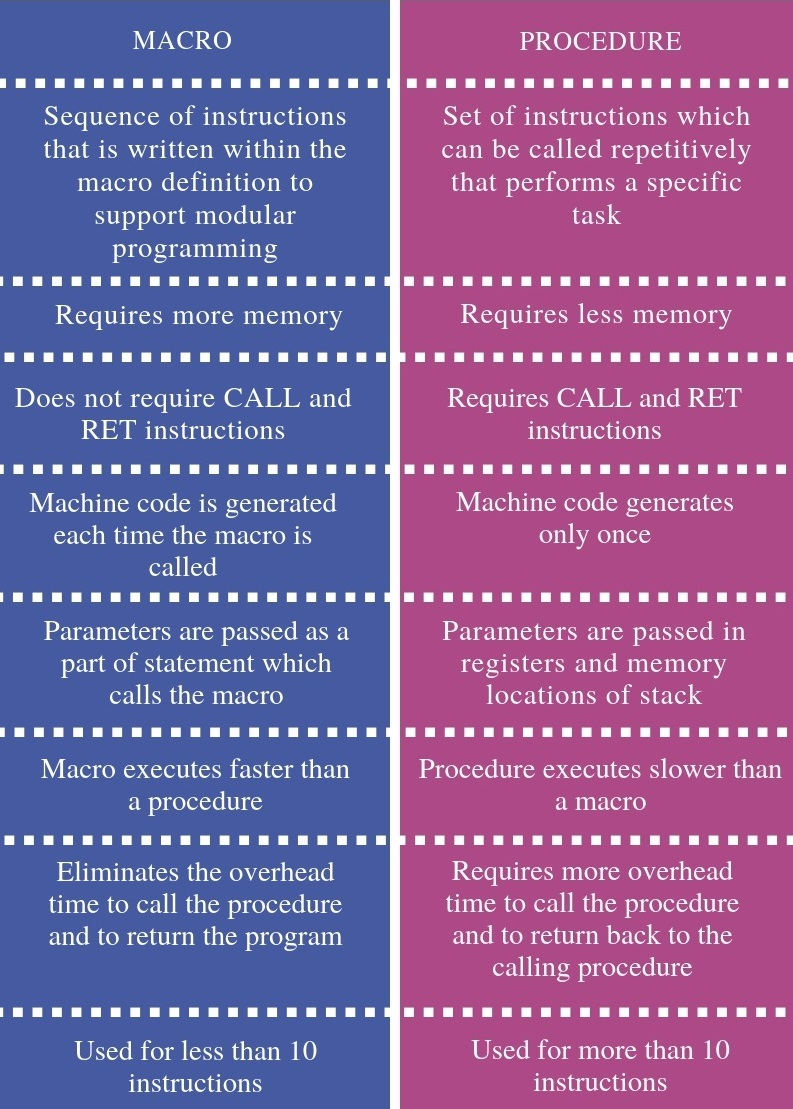
\includegraphics[width=14cm]{Macro-vs-Procedure.jpg}
        \caption{Difference between Macro and Procedure}
        \label{fig:vs}
\end{figure}

\end{document}
